\documentclass[t]{beamer}
\usepackage{beamerthemesplit}
\usepackage{pstricks}
\usepackage{graphicx}
\usepackage{hyperref}
\usepackage{listings}
\usepackage{subfigure}
\usepackage{multirow}
\usepackage{xspace}


\mode<presentation>
{ \usetheme{Boadilla}
  \setbeamercovered{transparent}
  \setbeamertemplate{items}[circle]
  \setbeamertemplate{theorems}[numbered]
  \setbeamertemplate{footline}[frame number]
}
 
%\useinnertheme[shadow=true]{rounded}
\useoutertheme{shadow}
\usecolortheme{whale}

\newcommand\blfootnote[1]{
  \begingroup
  \renewcommand\thefootnote{}\footnote{#1}
  \addtocounter{footnote}{-1}
  \endgroup
}

\mode
<all>

\def\answer{ANS}

\title{C Programming}
\author{WanLei Zhao}

\begin{document}
\begin{frame}
   \begin{center}
    \vspace{24pt}
    \Huge\textbf{C Programming}\blfootnote{Email: wlzhao@xmu.edu.cn, copyrights are fully preserved by the author.}\\
     \Huge{\mbox{Lab 1: }IDE for C coding}
    \vspace{36pt}
  \end{center}
  \begin{align*}
   \vspace{18pt}
      \large{\mbox{Lecturer:}~Dr.~\mbox{Wan-Lei~~Zhao}} \\
      \large{Spring~~Semester~~2022} \\
   \vspace{30pt}
  \end{align*}
\end{frame}

\definecolor{cornblue}{HTML}{6495ED}
\definecolor{navyblue}{HTML}{000080}
\definecolor{midnblue}{HTML}{191970}
\definecolor{lghtblue}{HTML}{B0C4DE}
\setbeamercolor{background}{fg=black, bg=lghtblue}
\setbeamercolor{palette primary}{fg=white, bg=lghtblue}
\setbeamercolor{palette secondary}{fg=black, bg=cornblue}
\setbeamercolor{palette tertiary}{fg=black, bg=lghtblue}
\setbeamercolor{palette quaternary}{fg=black, bg=lghtblue}
\setbeamercolor{frametitle}{fg=black, bg=white}
\definecolor{ballblue}{rgb}{0.13, 0.67, 0.8}
\definecolor{cornflowerblue}{rgb}{0.39,0.58,0.93}
\definecolor{babyblueeyes}{rgb}{0.63, 0.79, 0.95}

\setbeamertemplate{footline}
{
  \leavevmode%
  \hbox{%
  \begin{beamercolorbox}[wd=.275\paperwidth,ht=2.25ex,dp=1ex,center]{author in head/foot}%
    \usebeamerfont{author in head/foot}\insertshortauthor
  \end{beamercolorbox}%
  \begin{beamercolorbox}[wd=.44\paperwidth,ht=2.25ex,dp=1ex,center]{title in head/foot}%
    \usebeamerfont{title in head/foot}\insertshorttitle\hspace*{3em}
    \hspace*{1ex}
  \end{beamercolorbox}%
  \begin{beamercolorbox}[wd=.285\paperwidth,ht=2.25ex,dp=1ex,center]{date/foot}%
    \usebeamerfont{title in head/foot}\hspace*{2em}
    \insertframenumber{} / \inserttotalframenumber\hspace*{1ex}
  \end{beamercolorbox}}%
  \vskip0pt
}



% preset-listing options
\lstset{
  backgroundcolor=\color{white},   
  basicstyle=\footnotesize,    
  language=c,
  breakatwhitespace=false,         
  breaklines=true,                 % sets automatic line breaking
  captionpos=b,                    % sets the caption-position to bottom
  commentstyle=\color{ballblue},    % comment style
  extendedchars=true,              
  frame=single,                    % adds a frame around the code     
  keywordstyle=\color{blue},       % keyword style
  numbers=left,                    
  numbersep=5pt,                   
  numberstyle=\tiny\color{blue}, 
  rulecolor=\color{babyblueeyes},
  stepnumber=1,              
  stringstyle=\color{black},     % string literal style
  tabsize=4,                       % sets default tabsize to 4 spaces
  title=\lstname                   
}


%\section{VC++ 6.0 IDE}
%\label{sec:vc}
%\begin{frame}<beamer>
%    \frametitle{Outline}
%    \tableofcontents[currentsection]
%\end{frame}
%
%
%\begin{frame}{VC++ 6.0 IDE (1)}
%	\begin{figure}
%		\begin{center}
%			\begin{figure}
%				\includegraphics[width=0.8\linewidth]{figs/vc1.pdf}
%			\end{figure}
%		\end{center}
%	\end{figure}
%	\begin{itemize}
%		\item {Create/New a C project}
%	\end{itemize}
%\end{frame}
%
%\begin{frame}{VC++ 6.0 IDE (2)}
%	\begin{figure}
%		\begin{center}
%			\begin{figure}
%				\includegraphics[width=0.8\linewidth]{figs/vc2.pdf}
%			\end{figure}
%		\end{center}
%	\end{figure}
%	\begin{itemize}
%		\item {Choose to create "\textcolor{red}{Win32 Console Application}"}
%		\item {Give a meaningful name for your project, such as "test1"}
%	\end{itemize}
%\end{frame}
%
%\begin{frame}{VC++ 6.0 IDE (3)}
%	\begin{figure}
%		\begin{center}
%			\begin{figure}
%				\includegraphics[width=0.8\linewidth]{figs/vc3.pdf}
%			\end{figure}
%		\end{center}
%	\end{figure}
%	\begin{itemize}
%		\item {Choose to create "\textcolor{red}{an empty project}"}
%	\end{itemize}
%\end{frame}
%
%\begin{frame}{VC++ 6.0 IDE (4)}
%	\begin{figure}
%		\begin{center}
%			\begin{figure}
%				\includegraphics[width=0.8\linewidth]{figs/vc4.pdf}
%			\end{figure}
%		\end{center}
%	\end{figure}
%	\begin{itemize}
%		\item {Create C files under the your current project}
%		\item {Give a meaningful and unique name for your file}
%	\end{itemize}
%\end{frame}
%
%\begin{frame}{VC++ 6.0 IDE (5)}
%	\begin{figure}
%		\begin{center}
%			\begin{figure}
%				\includegraphics[width=0.8\linewidth]{figs/vc5.pdf}
%			\end{figure}
%		\end{center}
%	\end{figure}
%	\begin{itemize}
%		\item {Edit your current C file}
%		\item {Keywords are in \textcolor{blue}{blue}}
%	\end{itemize}
%\end{frame}
%
%\begin{frame}{VC++ 6.0 IDE (6)}
%	\begin{figure}
%		\begin{center}
%			\begin{figure}
%				\includegraphics[width=0.8\linewidth]{figs/vc6.pdf}
%			\end{figure}
%		\end{center}
%	\end{figure}
%	\begin{itemize}
%		\item {When there is something wrong during compiling}
%		\item {It will be shown in the window below}
%	\end{itemize}
%\end{frame}
%
%\begin{frame}{VC++ 6.0 IDE (7)}
%	\begin{figure}
%		\begin{center}
%			\begin{figure}
%				\includegraphics[width=0.8\linewidth]{figs/flow.pdf}
%			\end{figure}
%		\end{center}
%	\end{figure}
%\end{frame}
%
%\begin{frame}
%\frametitle{Hello world (1)}
%\begin{itemize}
%	\item {Try following code:}
%	\begin{enumerate}
%		\item {\#include $<$stdio.h$>$}
%		\item {int~main(~)}
%		\item {\{}
%		\item {~~~printf("Hello world$\setminus$n");}
%		\item {\}}
%	\end{enumerate}
%\end{itemize}
%\end{frame}
%
%\begin{frame}
%\frametitle{Hello world (2)}
%\begin{itemize}
%	\item {Try following code:}
%	\begin{enumerate}
%		\item {\#include $<$stdio.h$>$}
%		\item {int~main(~)}
%		\item {\{}
%		\item {~~~printf("Hello China$\setminus$n");}
%		\item {~~~printf("Hello world$\setminus$n");}
%		\item {~~~printf("Hello universe$\setminus$n");}
%		\item {\}}
%	\end{enumerate}
%\end{itemize}
%\begin{itemize}
%	\item {This is an experiment}
%	\item {Based on this great experiment, we know that}
%	\item {\textcolor{red}{Codes are executed from top to bottom}}
%\end{itemize}
%\end{frame}

\section{Codeblocks IDE}
\label{sec:cb}
\begin{frame}<beamer>
    \frametitle{Outline}
    \tableofcontents[currentsection]
\end{frame}

\begin{frame}{Codeblocks}
\begin{itemize}
	\item {It is free software, available at following link}
\end{itemize}
\begin{center}
\href{http://121.192.176.204/sourceforge.net/projects/codeblocks/files/Binaries/16.01/Windows/codeblocks-16.01mingw-setup.exe}{\textcolor{blue}{\underline{CodeBlocks 16.01 Windows binary}}}
\end{center}
\begin{itemize}
	\item {Lightweiht and stable}
	\item {Cross platform: Linux, Windows and MacOS}
\end{itemize}
\end{frame}

\begin{frame}{Compiler Setup}
	\begin{figure}
		\begin{center}
			\begin{figure}
				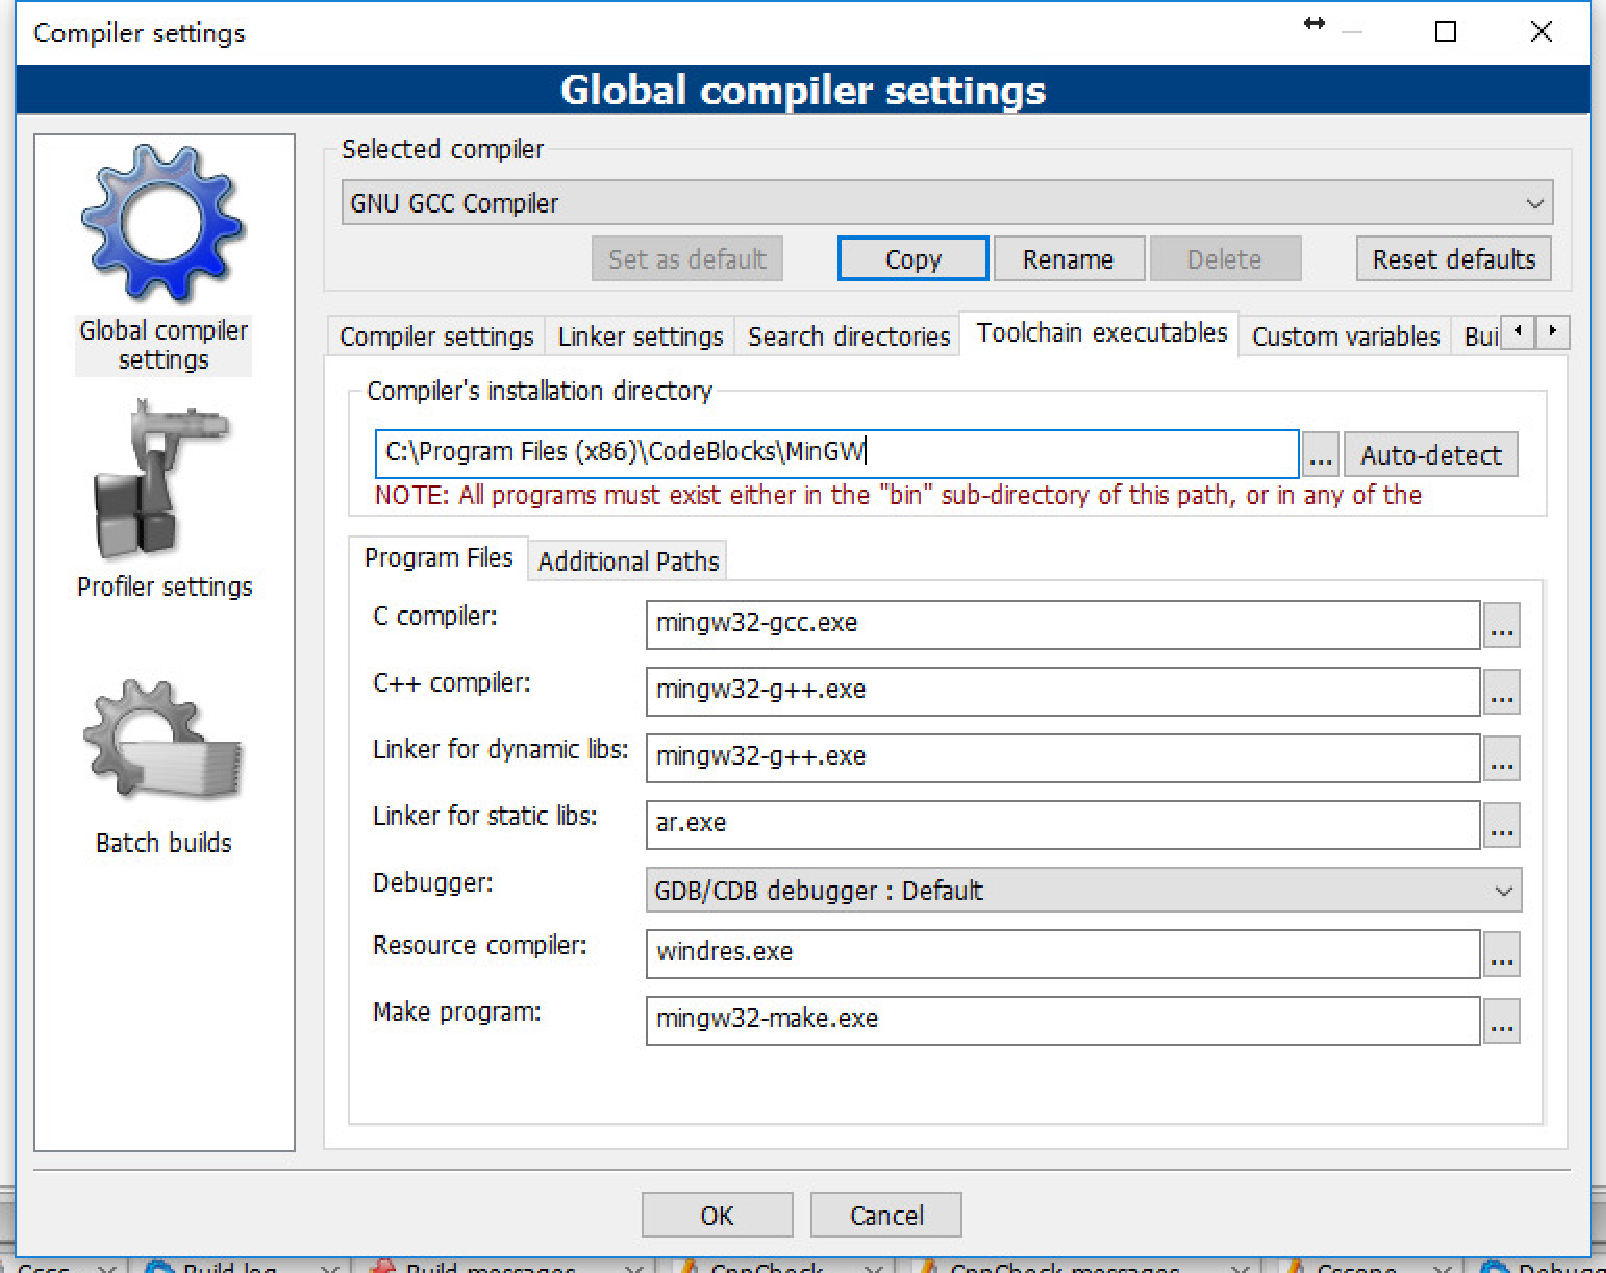
\includegraphics[width=0.6\linewidth]{figs/cbx0.pdf}
			\end{figure}
		\end{center}
	\end{figure}
	\begin{enumerate}
		\item {Go to menu: Settings$\rightarrow$Compiler Settings$\rightarrow$\textcolor{red}{Toolchain Executables}}
		\item {Type in the path for mingw compiler, e.g., C:/Program Files (x86)/CodeBlocks/MingW/}
	\end{enumerate}
	
\end{frame}


\begin{frame}{Create a project: step 1}
	\begin{figure}
		\begin{center}
			\begin{figure}
				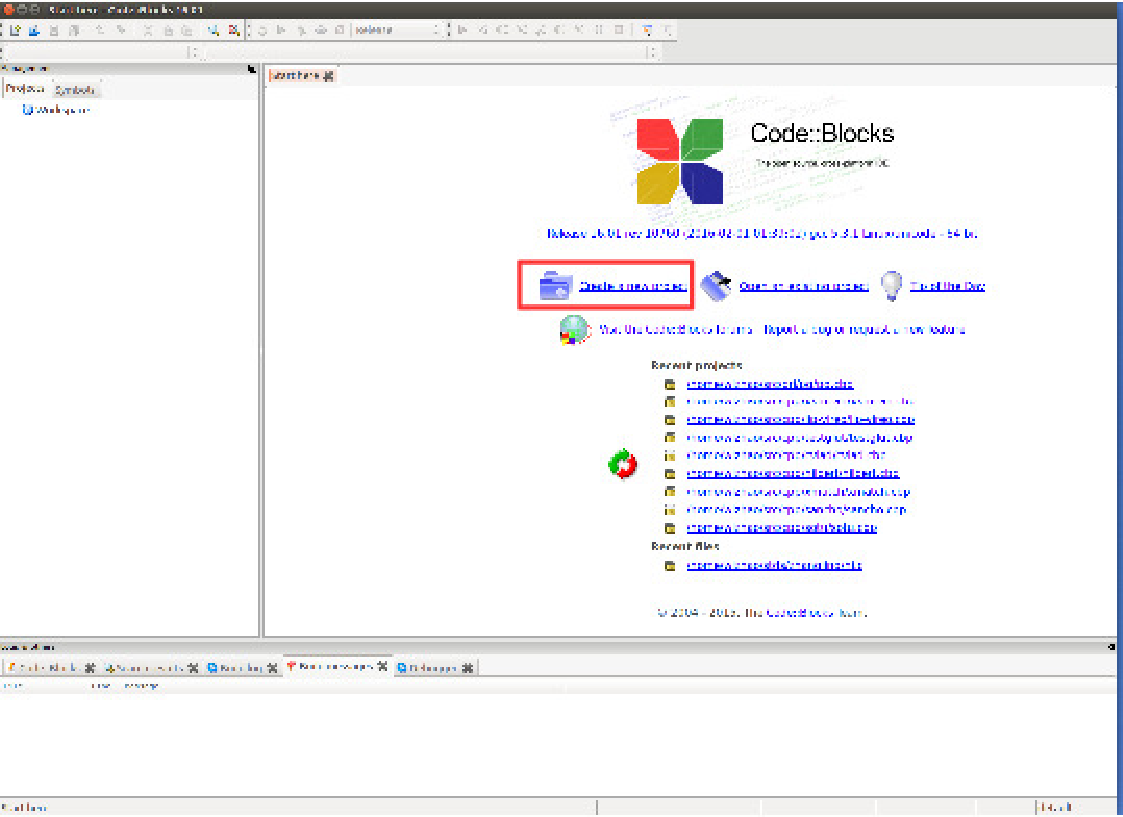
\includegraphics[width=0.8\linewidth]{figs/cbx1.pdf}
			\end{figure}
		\end{center}
	\end{figure}
	\begin{itemize}
		\item {Create/New a C project}
	\end{itemize}
\end{frame}

\begin{frame}{Create a project: step 2}
	\begin{figure}
		\begin{center}
			\begin{figure}
				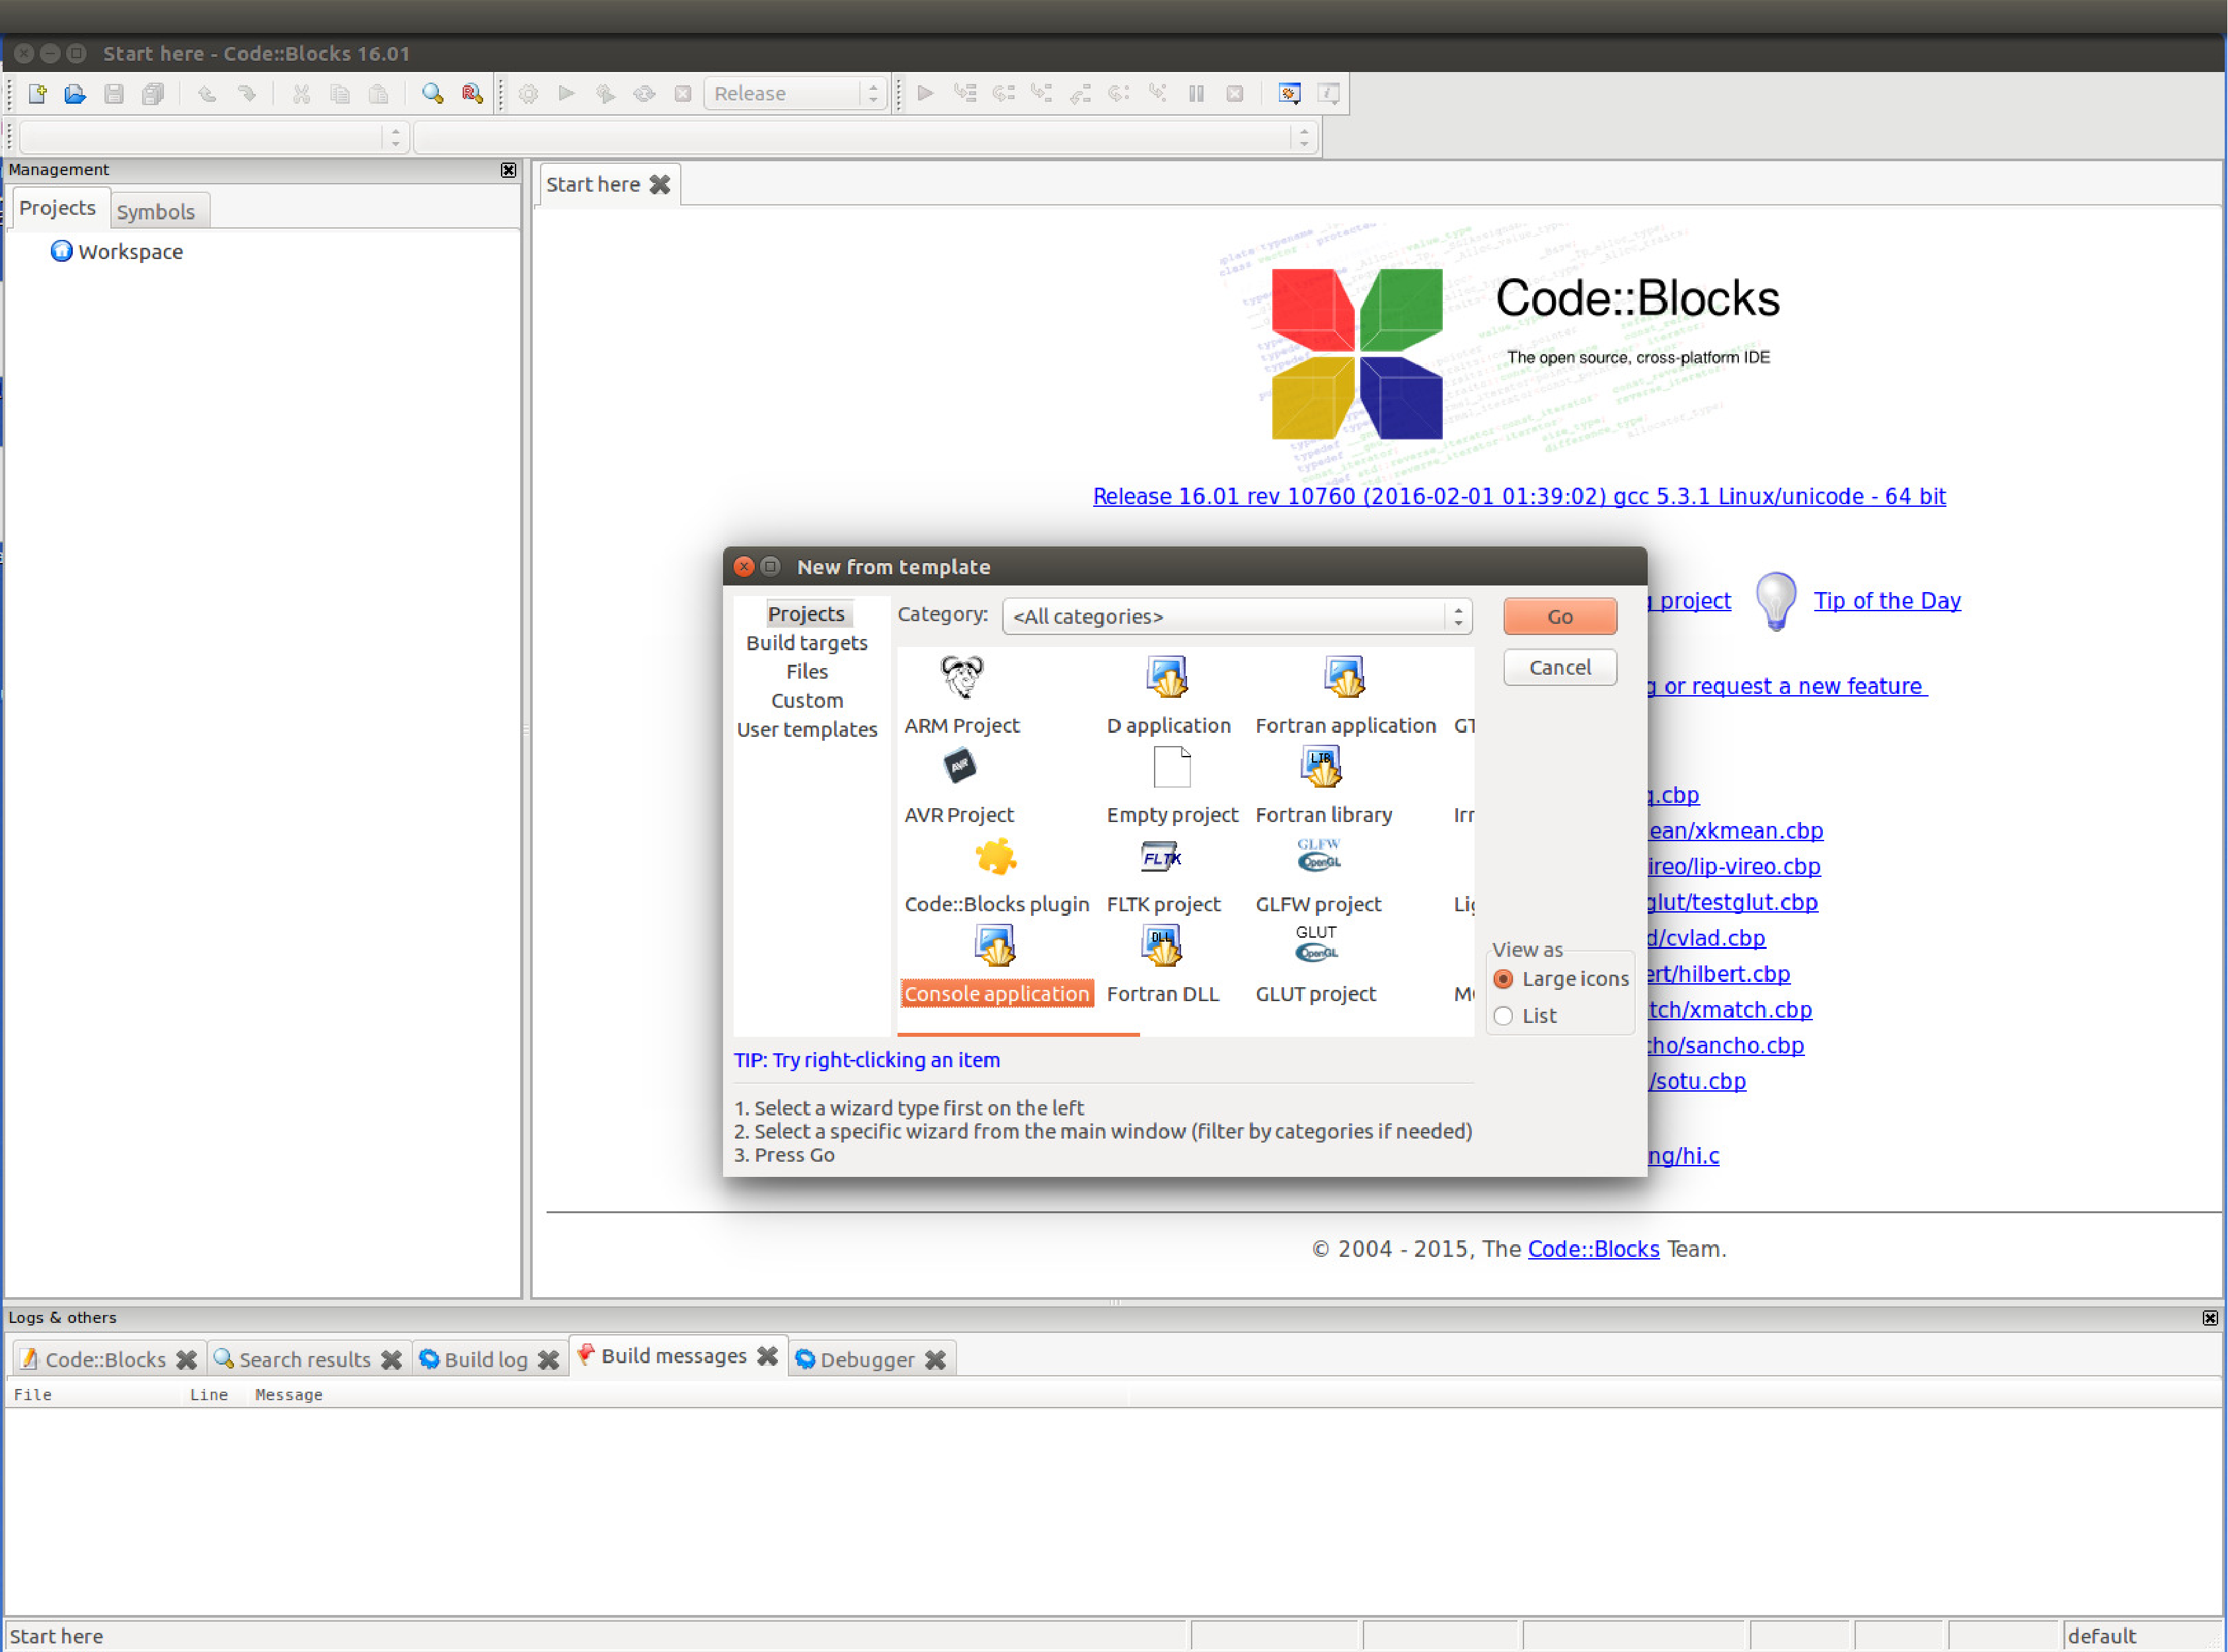
\includegraphics[width=0.8\linewidth]{figs/cb2.pdf}
			\end{figure}
		\end{center}
	\end{figure}
	\begin{itemize}
		\item {Choose project type ``Console application''}
	\end{itemize}
\end{frame}

\begin{frame}{Create a project: step 3}
	\begin{figure}
		\begin{center}
			\begin{figure}
				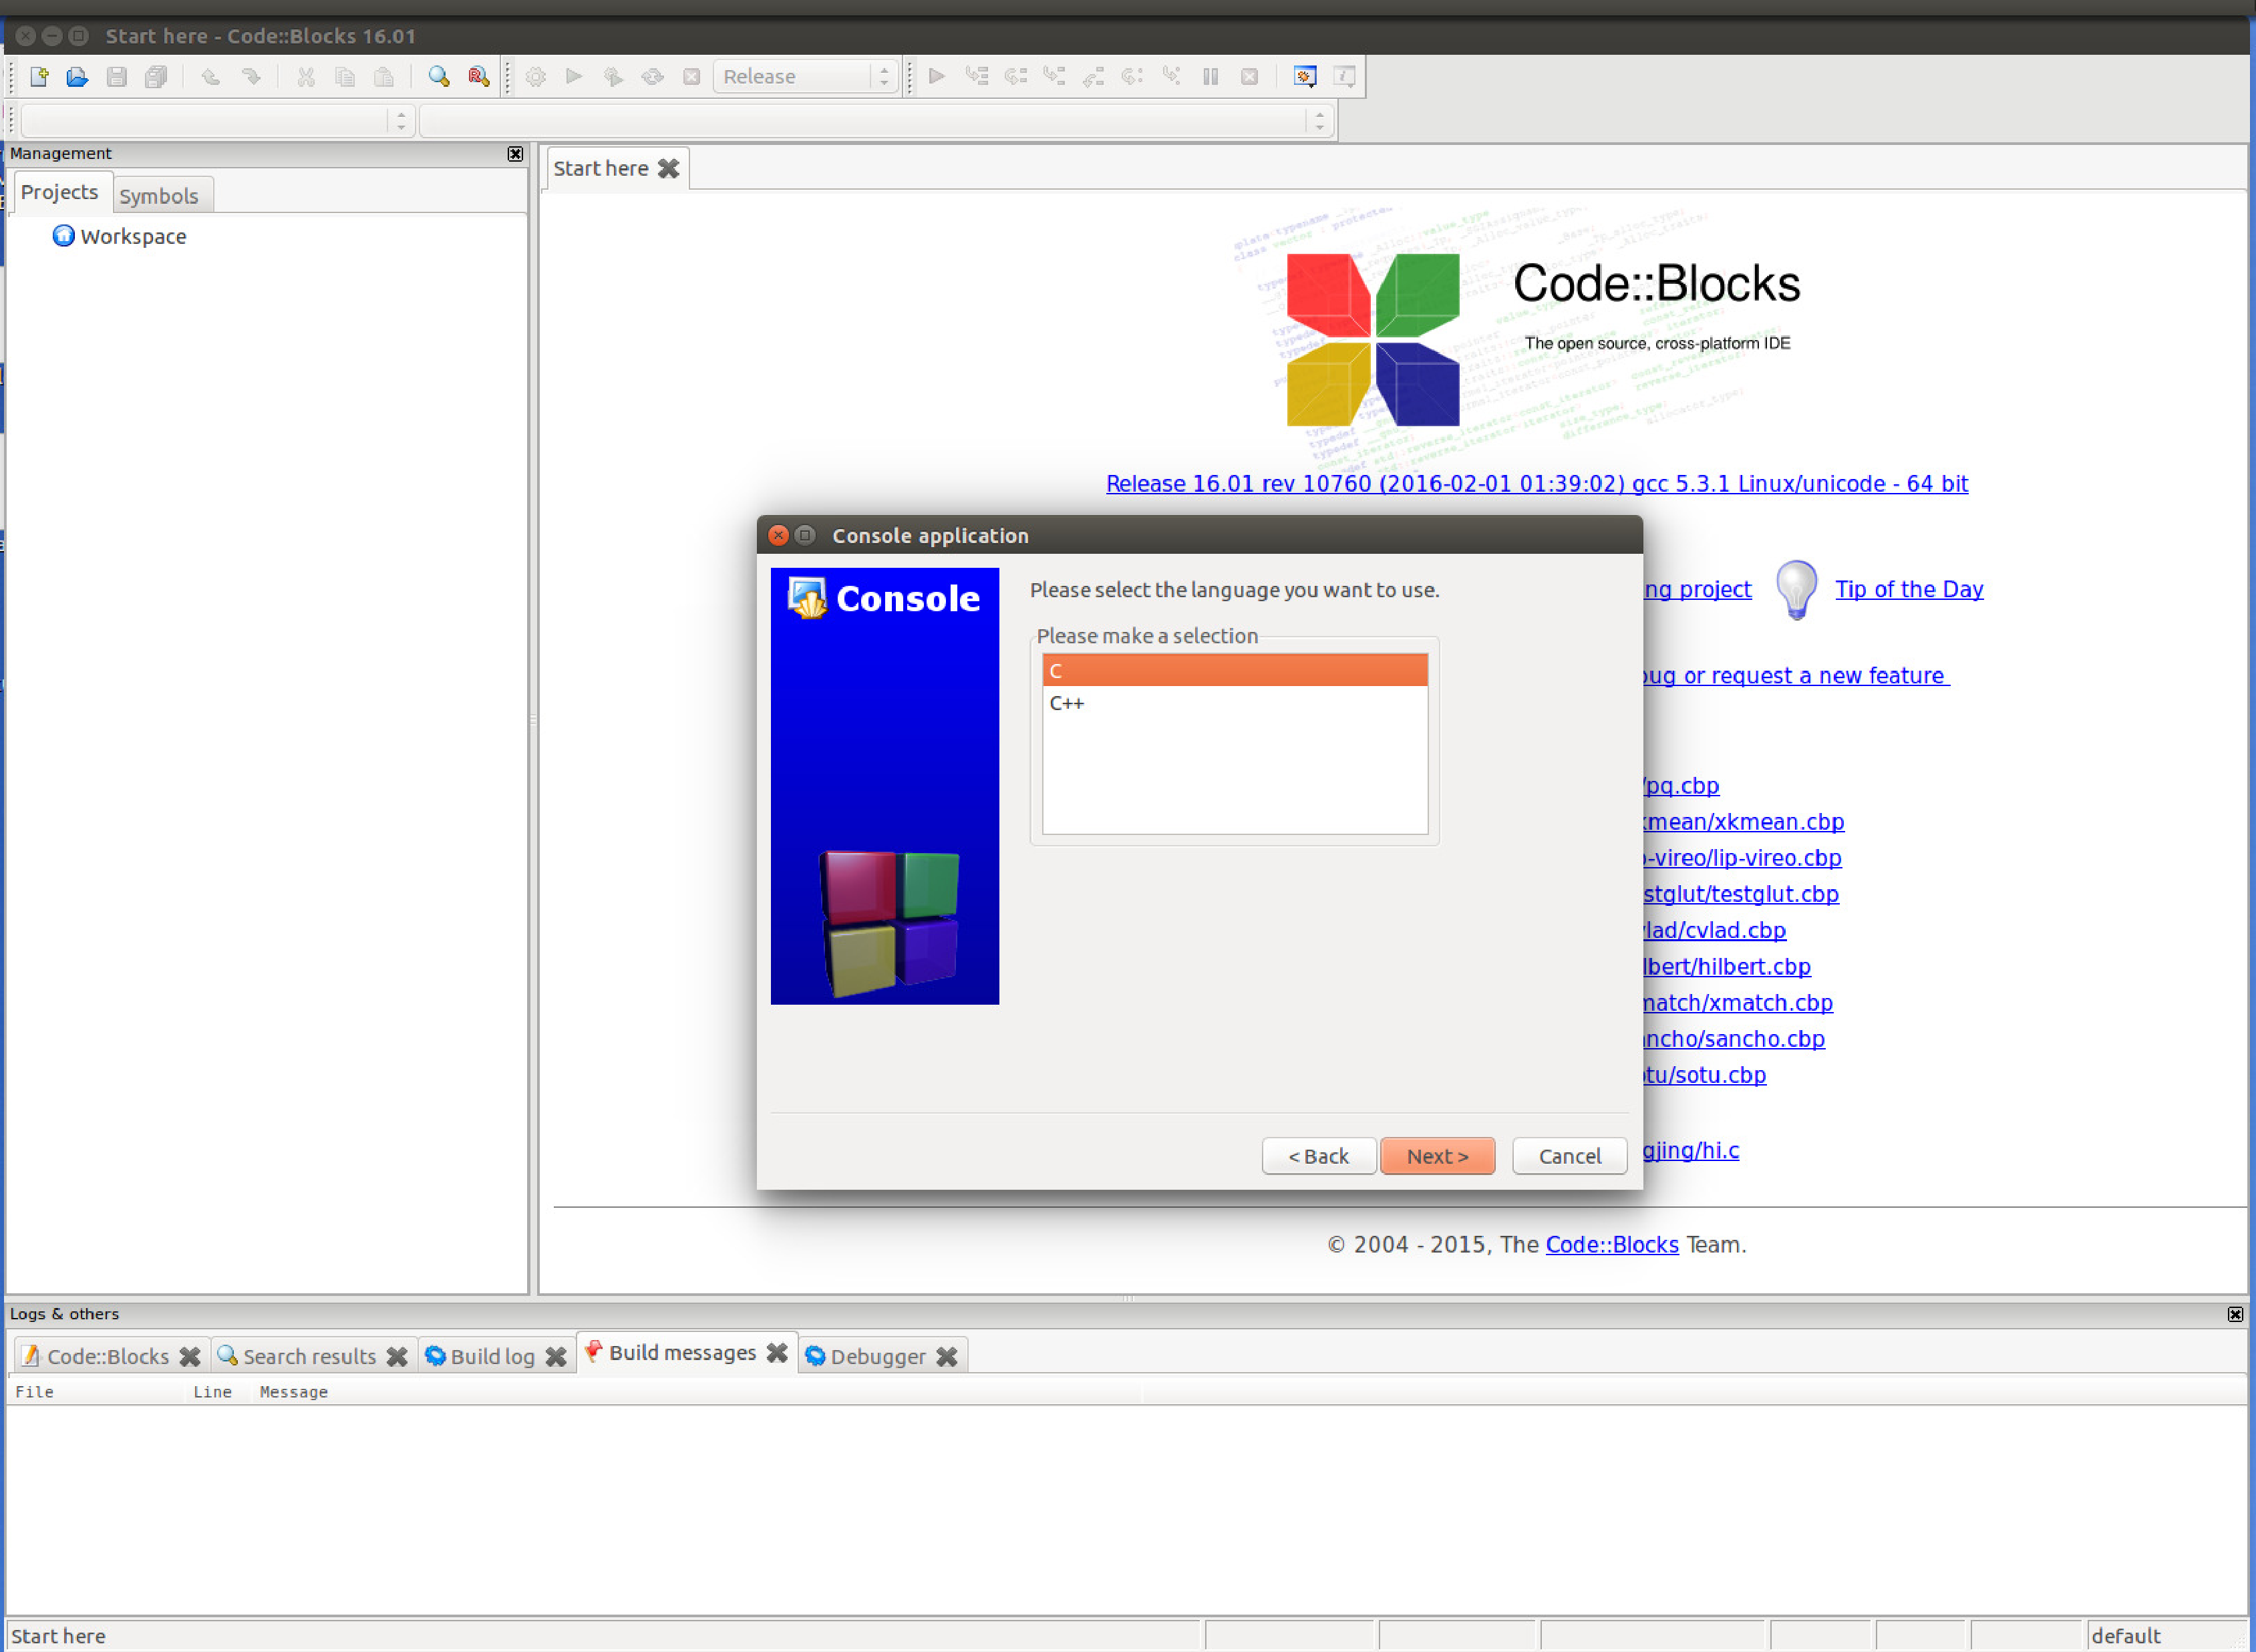
\includegraphics[width=0.8\linewidth]{figs/cb3.pdf}
			\end{figure}
		\end{center}
	\end{figure}
	\begin{itemize}
		\item {Set it as a ``C'' project}
	\end{itemize}
\end{frame}

\begin{frame}{Create a project: step 4}
	\begin{figure}
		\begin{center}
			\begin{figure}
				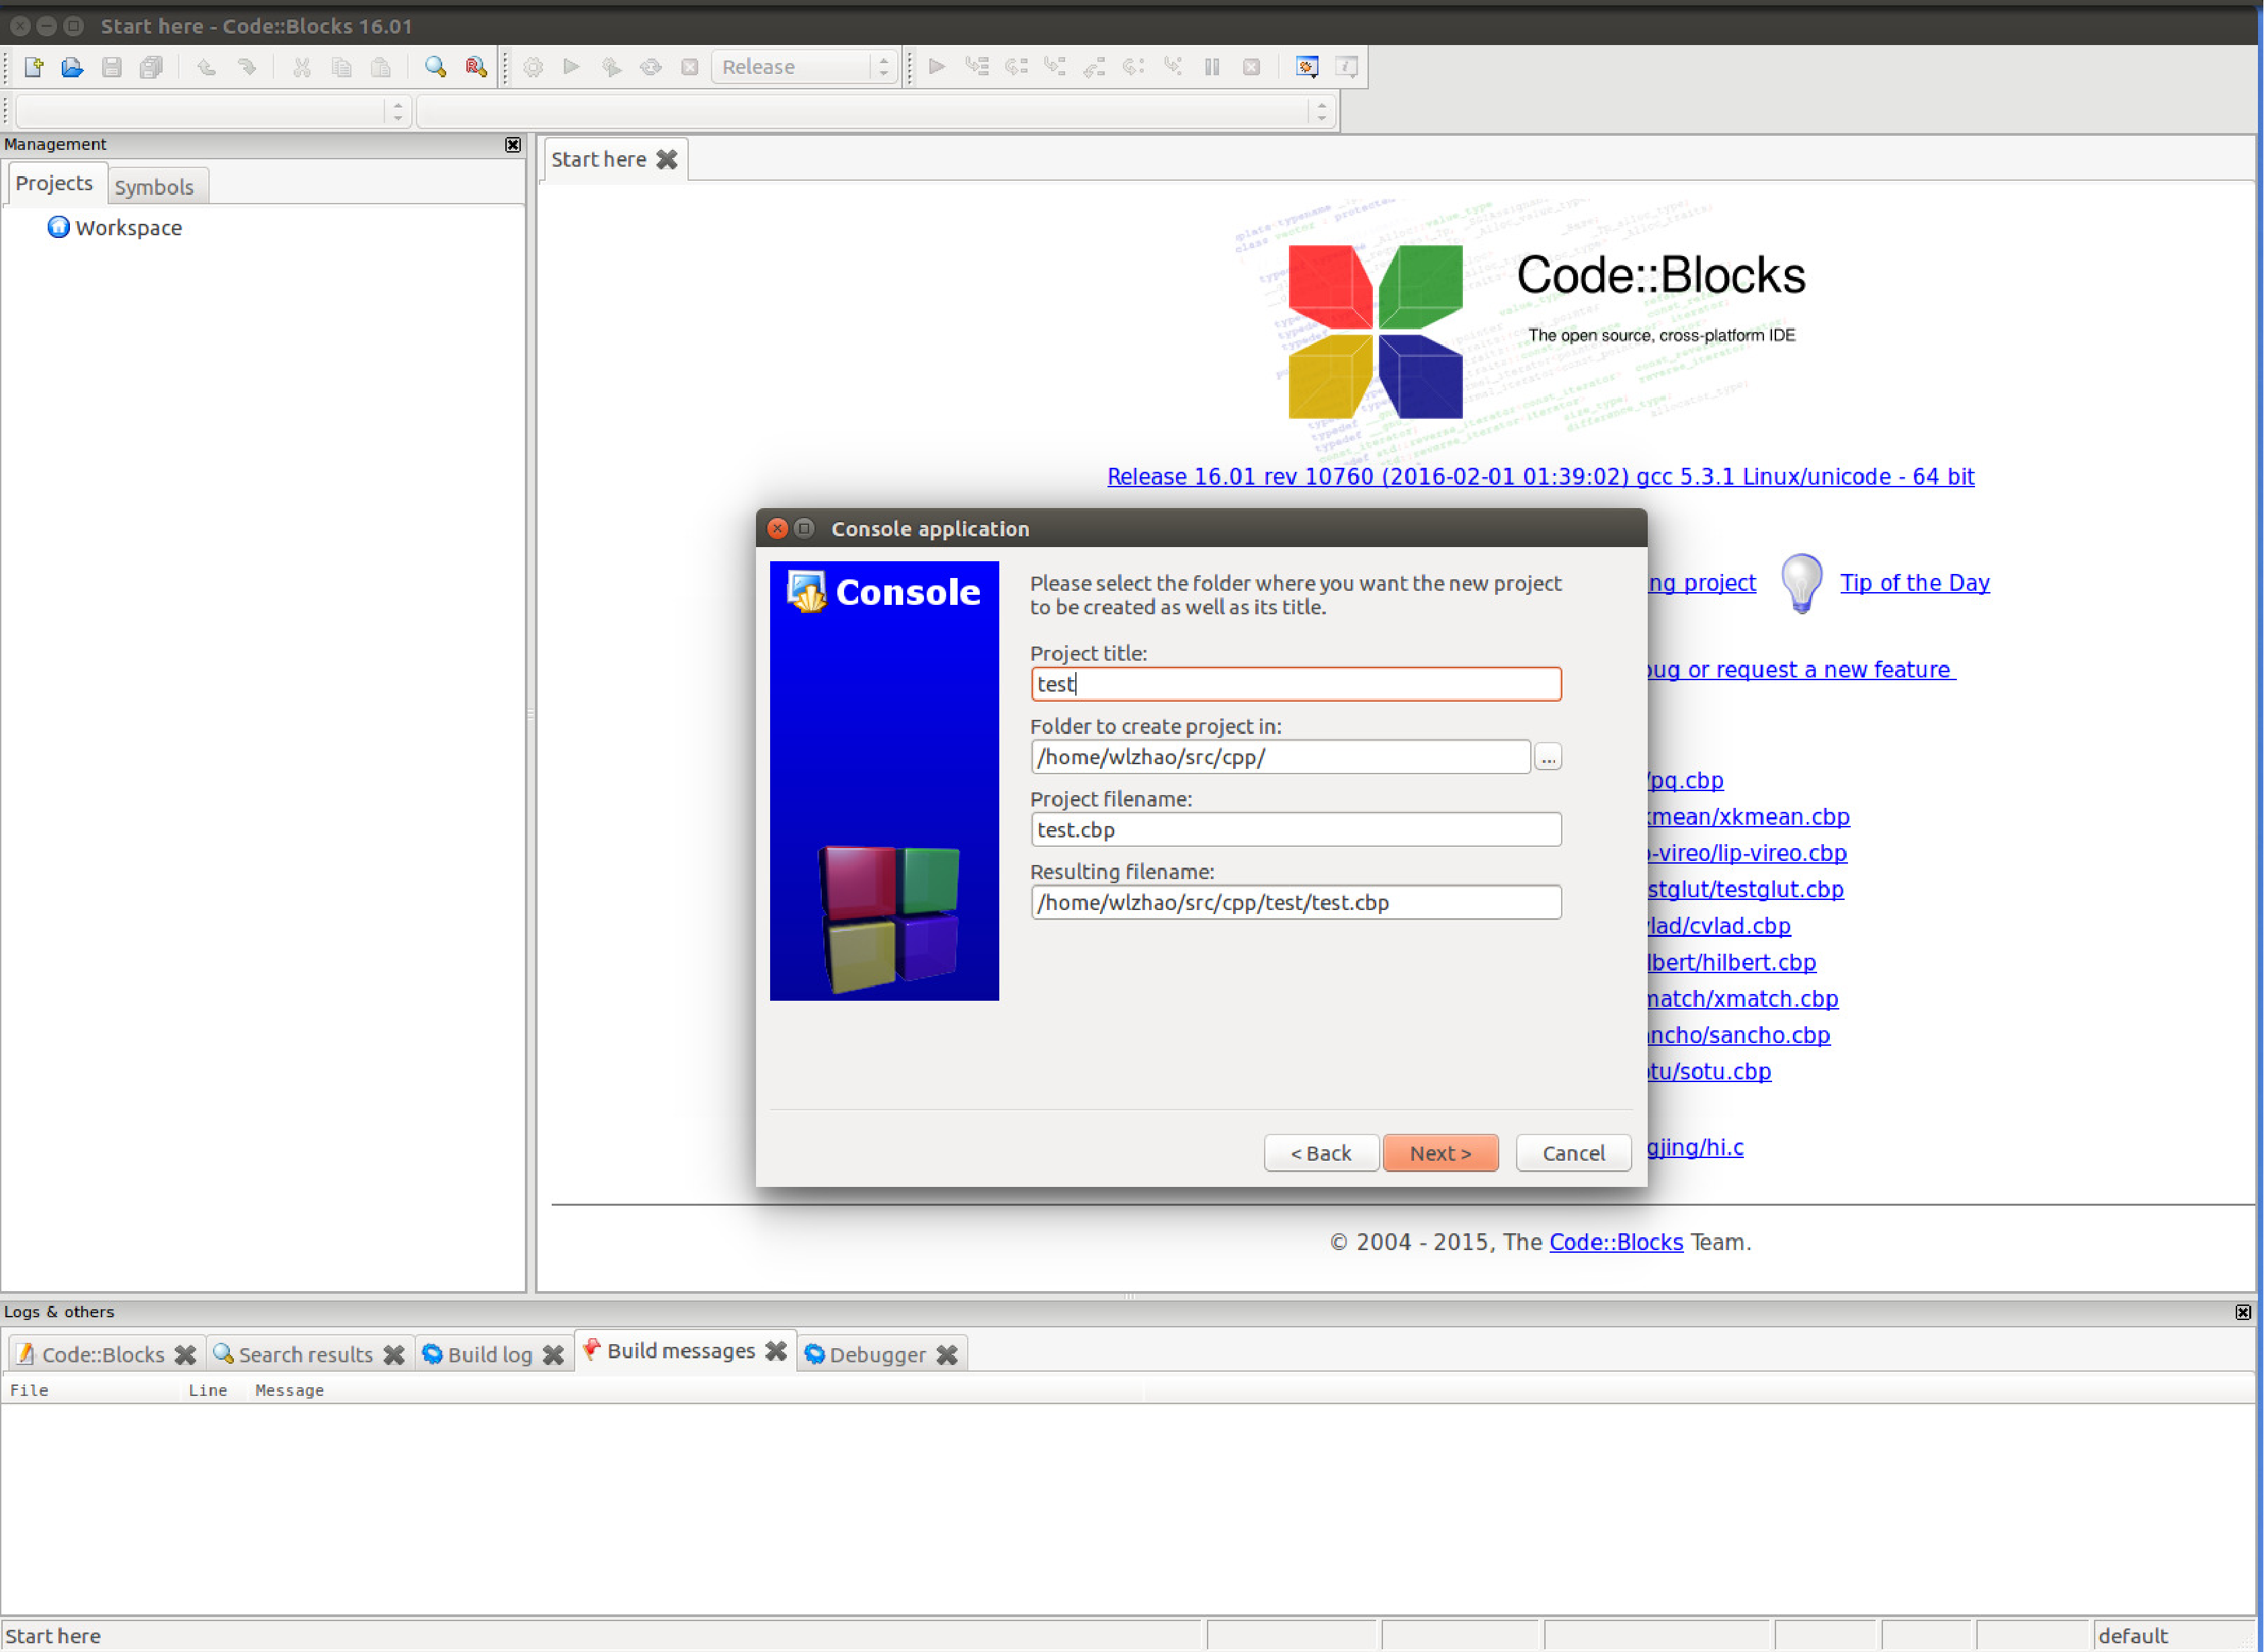
\includegraphics[width=0.8\linewidth]{figs/cb4.pdf}
			\end{figure}
		\end{center}
	\end{figure}
	\begin{itemize}
		\item {Give a name for your project}
	\end{itemize}
\end{frame}

\begin{frame}{Create a project: step 5}
	\begin{figure}
		\begin{center}
			\begin{figure}
				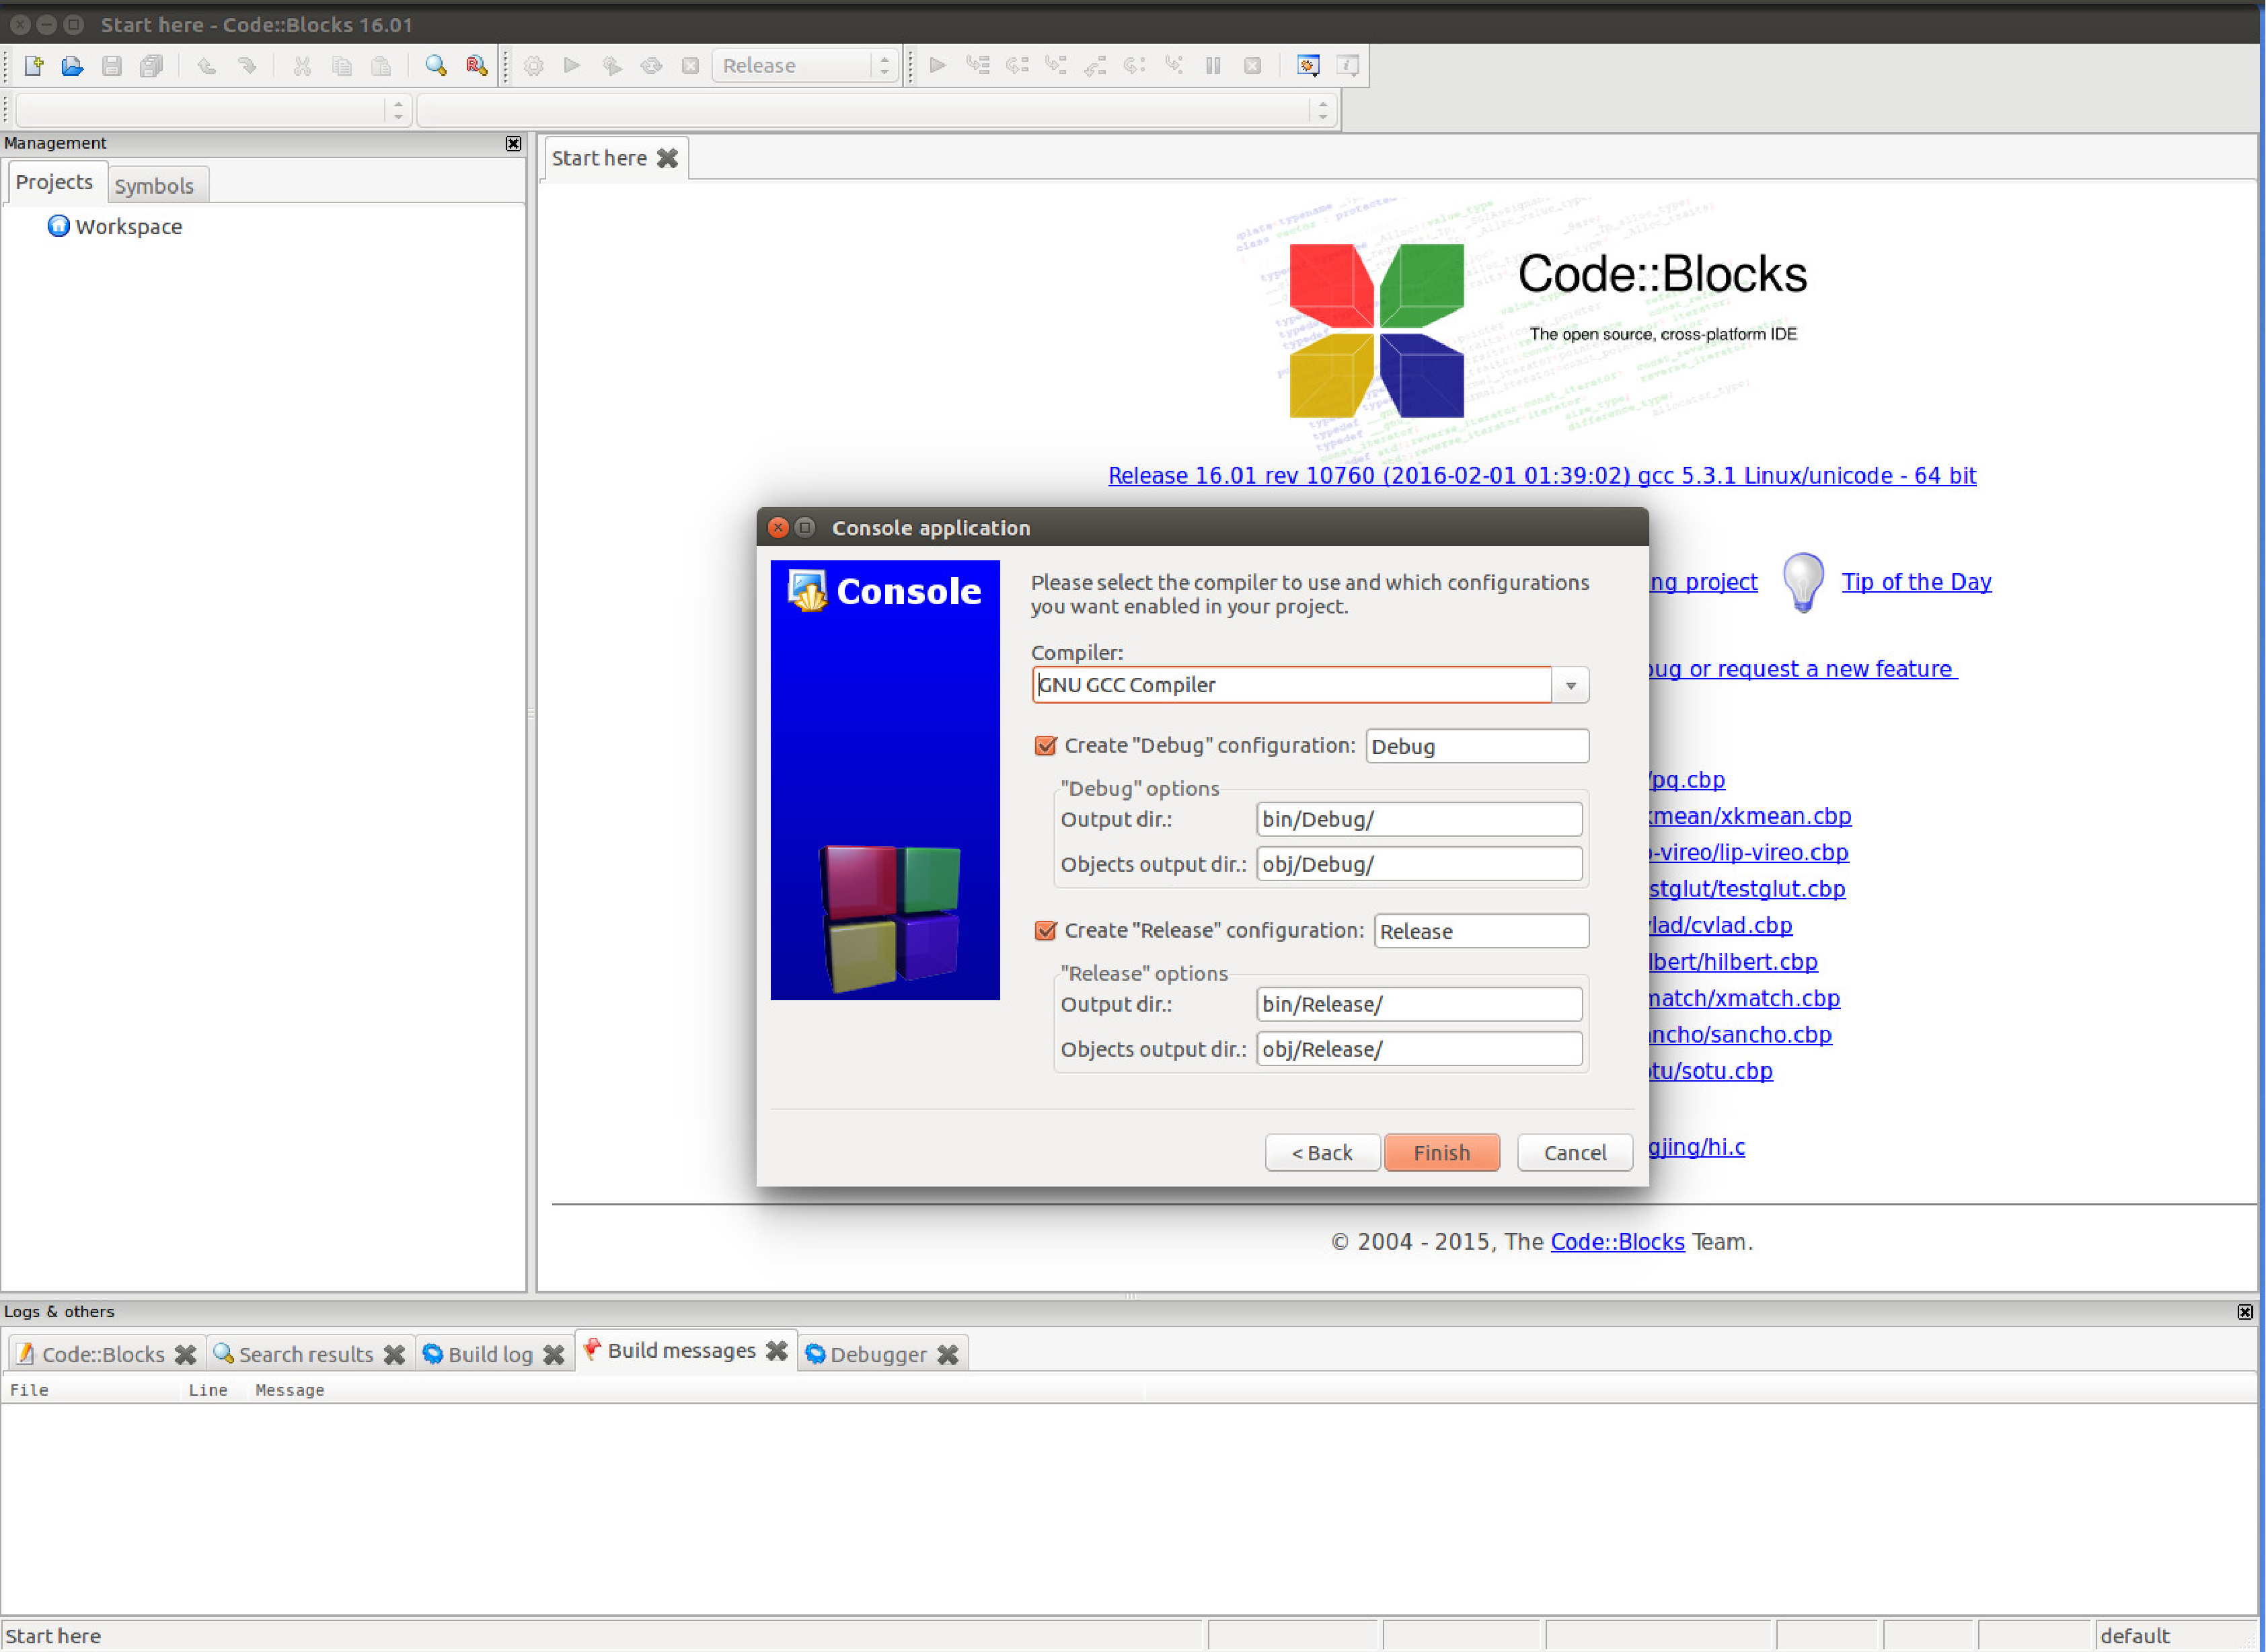
\includegraphics[width=0.8\linewidth]{figs/cb5.pdf}
			\end{figure}
		\end{center}
	\end{figure}
	\begin{itemize}
		\item {Choose ``C'' compiler for your project}
	\end{itemize}
\end{frame}

\begin{frame}{Create a project: step 6}
	\begin{figure}
		\begin{center}
			\begin{figure}
				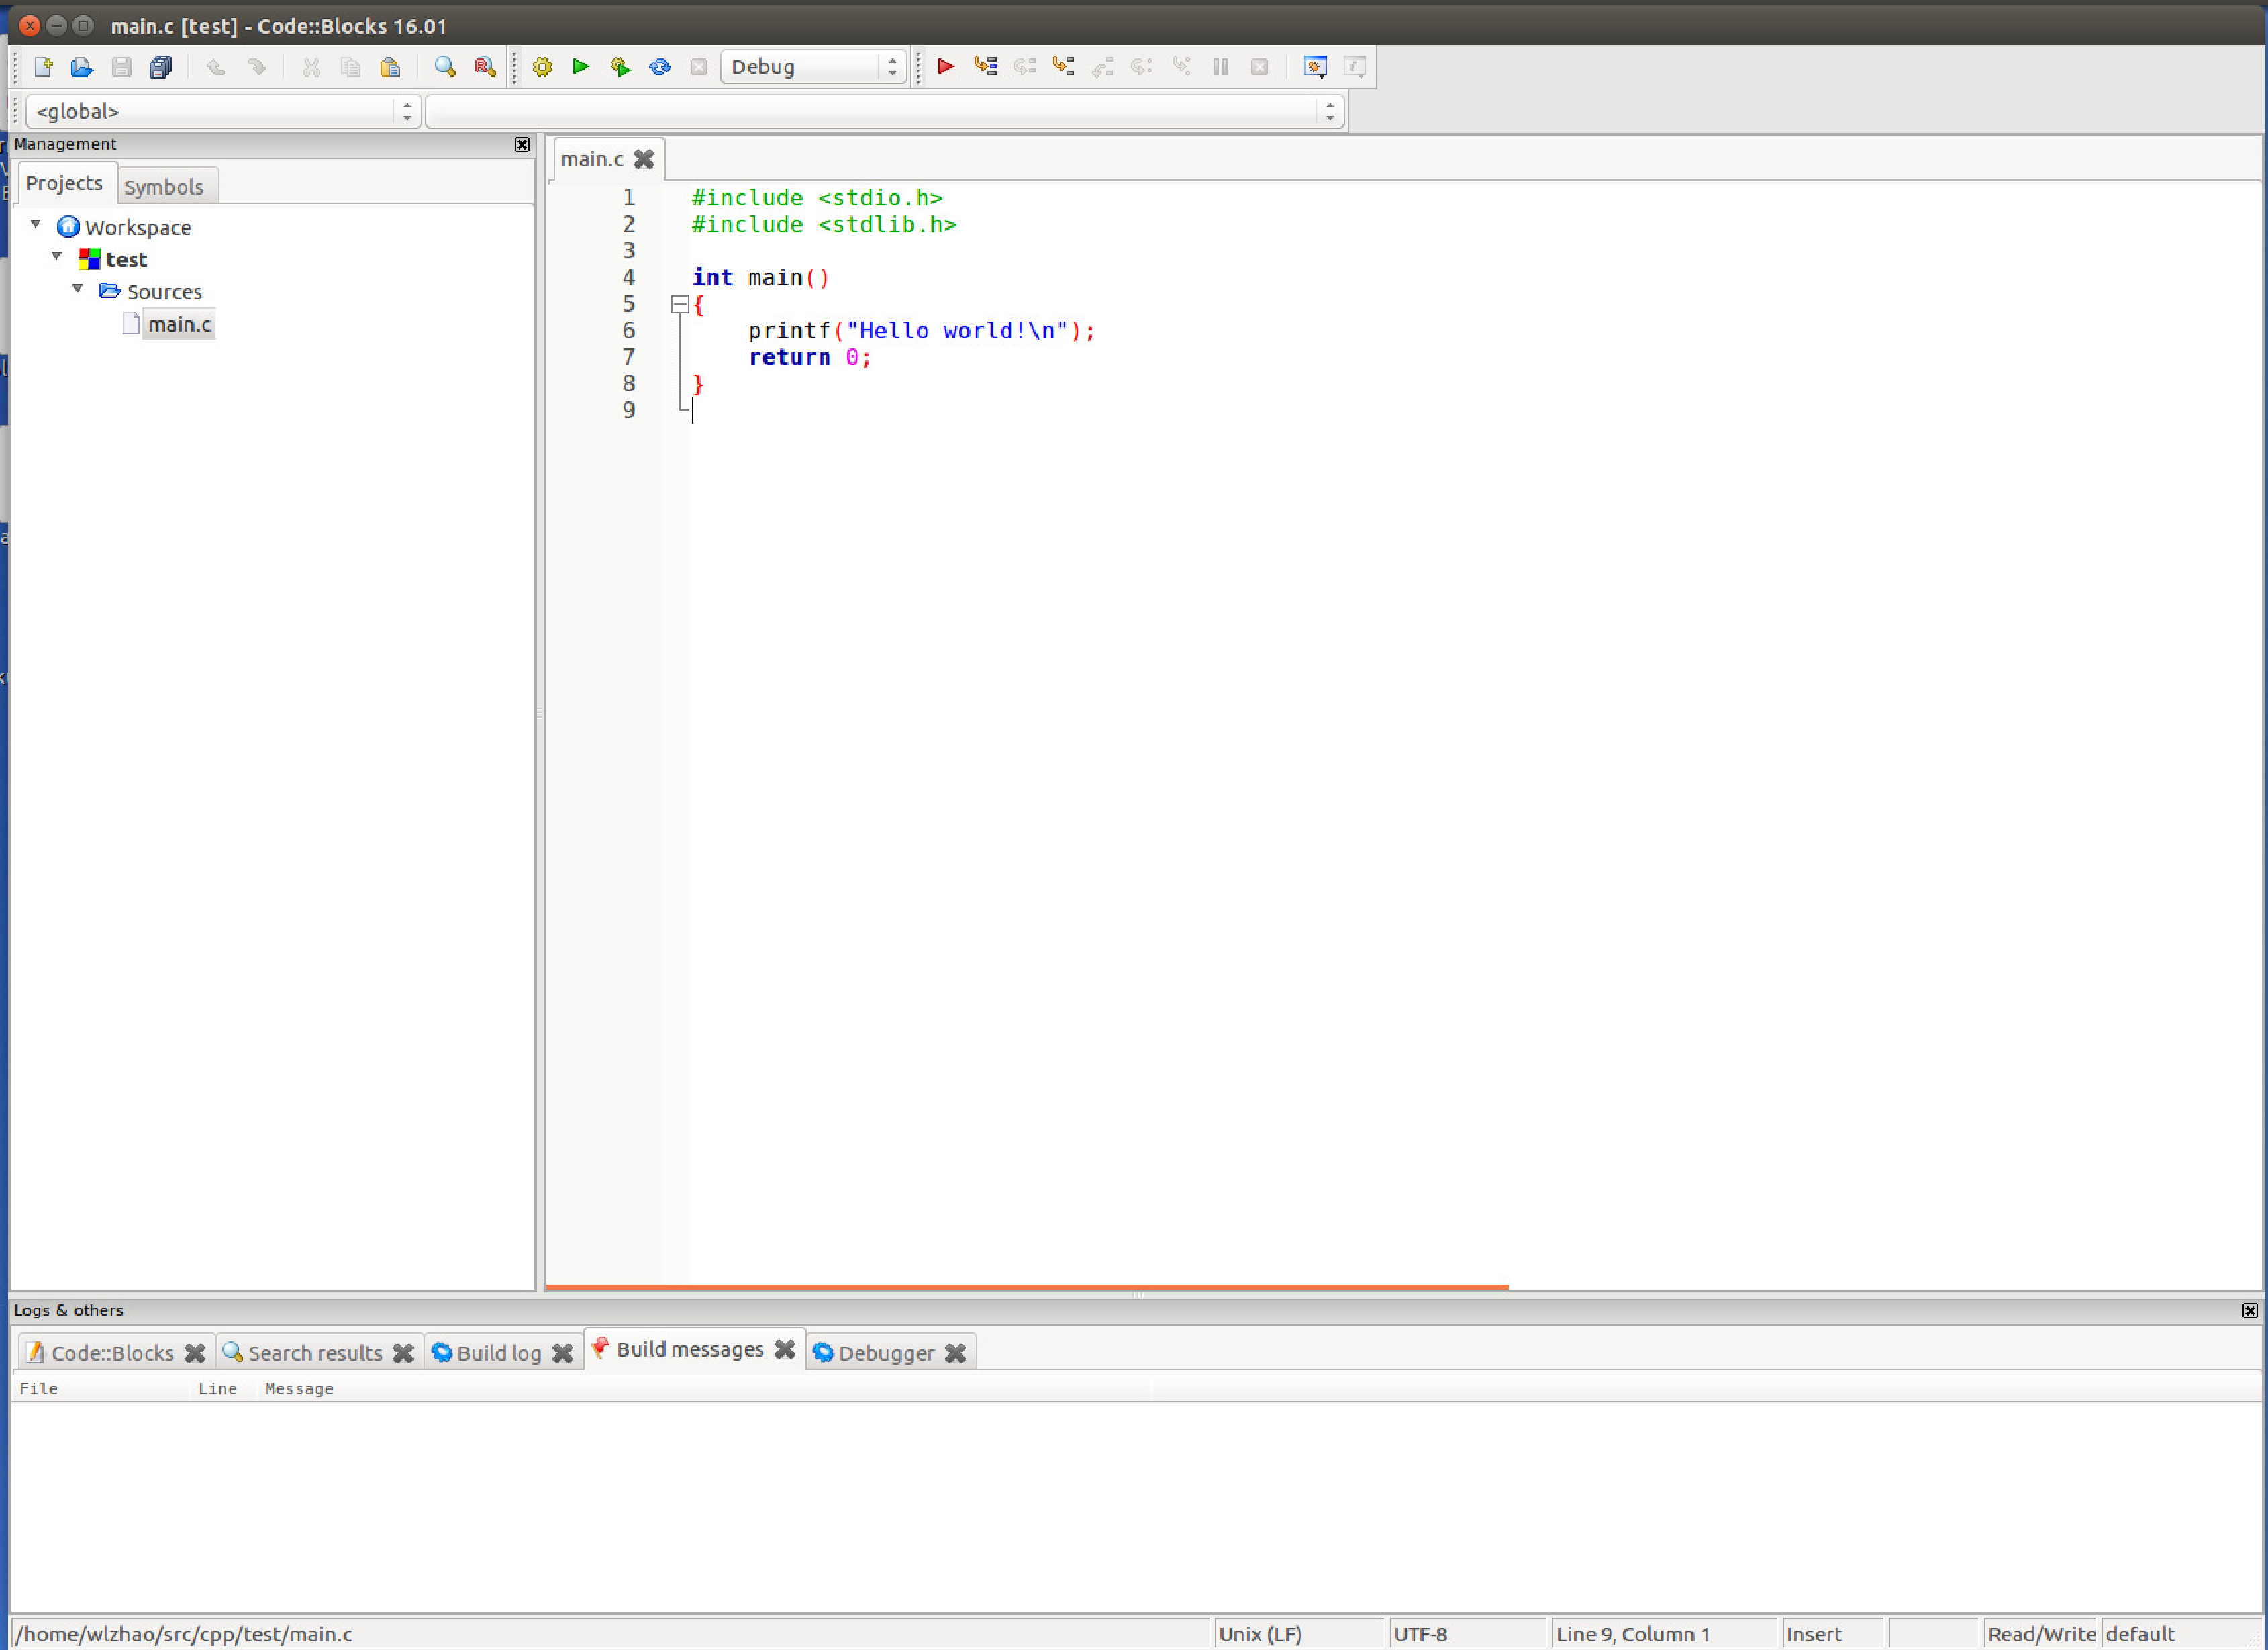
\includegraphics[width=0.8\linewidth]{figs/cb6.pdf}
			\end{figure}
		\end{center}
	\end{figure}
	\begin{itemize}
		\item {Start to work with your project}
	\end{itemize}
\end{frame}

\section{Visual Studio Code}
\label{sec:vs}
\begin{frame}{Main interface of VS code}
	\begin{figure}
		\begin{center}
			\begin{figure}
				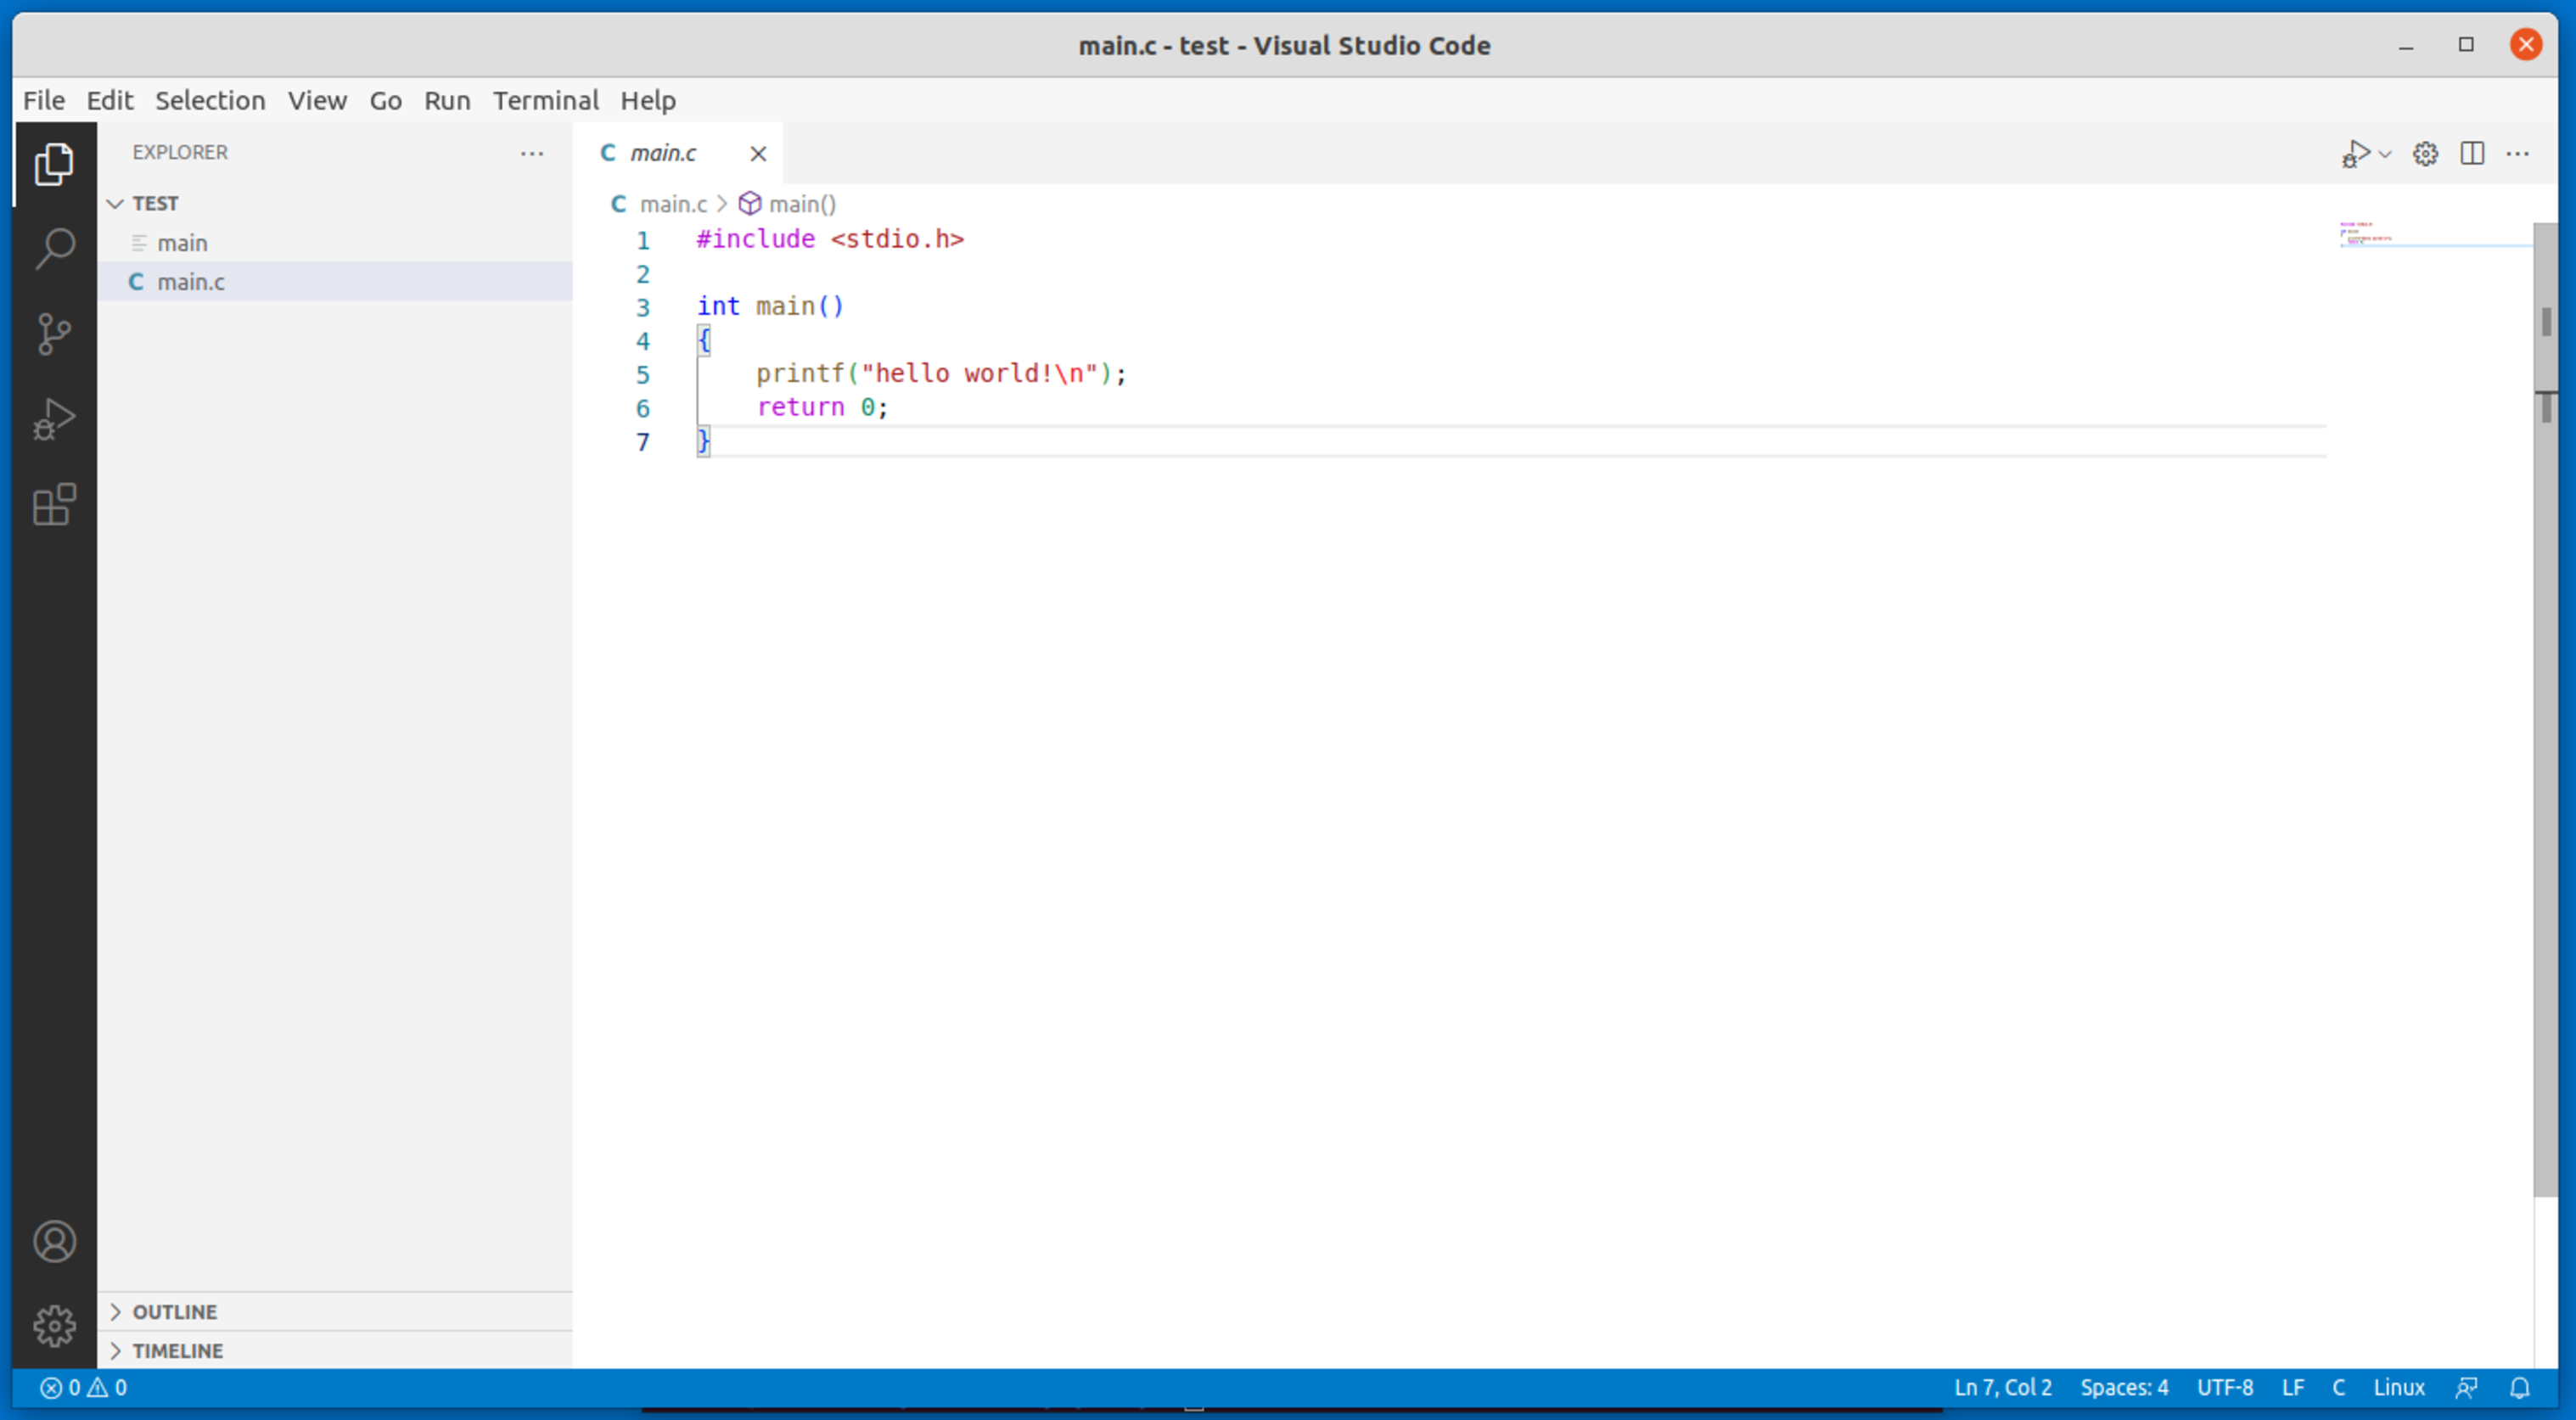
\includegraphics[width=0.8\linewidth]{figs/vscode.pdf}
			\end{figure}
		\end{center}
	\end{figure}
	\begin{itemize}
		\item {VS code is the most powerful and convenient Editor\footnote{https://code.visualstudio.com/download}}
		\item {One editor for designed for various programming languages, C, C++, Python and Java, etc}
	\end{itemize}
\end{frame}

\section{Variables}
\label{sec:var}
\begin{frame}<beamer>
    \frametitle{Outline}
    \tableofcontents[currentsection]
\end{frame}

\begin{frame}[fragile]
\frametitle{Variable Types and Operations}
\begin{itemize}
	\item {Try following code:}
\begin{lstlisting}[xleftmargin=0.05\linewidth, linewidth=0.9\linewidth]
#include <stdio.h>
int main( )
{
  int a = 5, b = 3;
  float val1 = a/b;
  float val2 = (float)(a/b);
  float val3 = (float)(a+0.0)/b;
  printf("a/b is: val1 = %f\n", val1);
  printf("a/b is: val2 = %f\n", val2);
  printf("a/b is: val3 = %f\n", val3);
}
\end{lstlisting}
\end{itemize}
\end{frame}

\begin{frame}[fragile]
\frametitle{Character and String}
\vspace{-0.14in}
\begin{itemize}
	\item {Try following code:}
\begin{lstlisting}[xleftmargin=0.05\linewidth, linewidth=0.9\linewidth]
#include <stdio.h>
int main()
{
   char *str1 = "abc\0de";
   char *str2 = "abc\rde";
   char *str3 = "abc\tde";
   char *str4 = "abc\t\b\b\b\b\bde";
   char ch1 = 'A'+6;
   char ch2 = 'A' + 'B';
   printf("%s\n", str1);
   printf("%s\n", str2);
   printf("%s\n", str3);
   printf("%s\n", str4);
   printf("%c, value=%d\n", ch1, ch1);
   printf("%c, value=%d\n", ch2, ch2);
}
\end{lstlisting}
\end{itemize}
\end{frame}

\begin{frame}[fragile]{How Variable Behaves}
\begin{itemize}
	\item {Guess the values of \textbf{a}, \textbf{i} and \textbf{j}}
	\item {Try following code to verify your answer:}
\end{itemize}

\begin{lstlisting}
#include <stdio.h>
int main()
{
   int  i = 4, j = 6;
   int  a = i + j;
   printf("a = %d\n", a);
   i = j - i; 
   j = i + j;
   printf("i = %d, j = %d\n", i, j);
}
\end{lstlisting}
\end{frame}

\begin{frame}[fragile]
\frametitle{printf() and Precision Control}
\begin{itemize}
	\item {Given float number \textcolor{red}{a = 231.36952}, integer number \textcolor{red}{b = 39} and integer number \textcolor{red}{c=0xEE}}
	\begin{enumerate}
		\item{Print out \textcolor{red}{a} with \textcolor{red}{2} digits precision and \textcolor{red}{3} digits precision respectively}
		\item{Print out octal and hexadecimal values of \textcolor{red}{b}}
		\item{Print out decimal and octal nunmber of \textcolor{red}{c}}
	\end{enumerate}
\end{itemize}

\begin{lstlisting}[xleftmargin=0.08\linewidth, linewidth=0.9\linewidth]
#include <stdio.h>
int main( )
{
   float a = 231.36952;
   int b = 39;
   int c = 0xEE;
}
\end{lstlisting}
\end{frame}

\ifx\answer\undefined
\begin{frame}[fragile]
\frametitle{printf() and Precision Control: the answer}
\begin{itemize}
	\item {Try following code:}
	\begin{lstlisting}[xleftmargin=0.08\linewidth, linewidth=0.9\linewidth]
#include <stdio.h>
int main( )
{
   float a = 231.36952;
   int b = 39;
   int c = 0xEE;
   printf("a = %3.2f\n", a);
   printf("a = %3.3f\n", a);
   printf("b = %0x\n", b);
   printf("b = %o\n",  b);
   printf("c = %d\n", c);
   printf("c = %o\n", c);
}
	\end{lstlisting}
\end{itemize}
\end{frame}
\fi

\begin{frame}[fragile]
\frametitle{Print out the values of different variables}
\vspace{-0.1in}
\begin{itemize}
	\item {Given following variables have been defined}
	\item {Please show the number of bytes they occupy in the memory}
\end{itemize}
\begin{lstlisting}[xleftmargin=0.08\linewidth, linewidth=0.96\linewidth]
#include <stdio.h>
int main()
{
   char ch = 'B';
   int  a  = 0;
   short b = 1024;
   double c = 0.1;
   float d = 22;
   double e = 3.1415926;
}
\end{lstlisting}
\vspace{-0.2in}
\begin{itemize}
	\item {Please print the values of different variables on the screen}
	\item {For example,}
\end{itemize}
\begin{lstlisting}[xleftmargin=0.08\linewidth, linewidth=0.96\linewidth]
   printf("%f\n", d);
\end{lstlisting}
\end{frame}

%\ifx\answer\undefined
\begin{frame}[fragile]
\frametitle{Precision of \textcolor{blue}{float} and \textcolor{blue}{double}}
\vspace{-0.1in}
\begin{lstlisting}[xleftmargin=0.08\linewidth, linewidth=0.96\linewidth]
#include <stdio.h>
int main()
{
   double c = 0.1;
   float d = 22;
   double e = 3.1415926;
   printf("e = %1.4lf\n", e);
   printf("e = %1.3lf\n", e);
   printf("e = %1.2lf\n", e);
}
\end{lstlisting}
\end{frame}
%\fi

\begin{frame}[fragile]{Print integer numbers with formating}
\begin{itemize}
	\item {Print out a=234, b=5, c=123, d=55, two numbers in each line}
	\item {Numbers are separated by `, '}
	\item {Each number occupy 6 digital position, right-aligned}
\end{itemize}
\begin{figure}
	\centering
	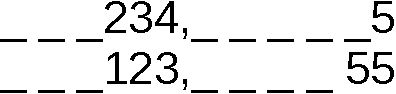
\includegraphics[width=0.5\linewidth]{figs/format.pdf}
\end{figure}
\end{frame}

%\ifx\answer\undefined
\begin{frame}[fragile]{Print integer numbers with right-aligned}
\begin{itemize}
	\item {Try following code:}
\end{itemize}

\begin{lstlisting}
#include <stdio.h>
int main()
{
   int a = 234;
   int b = 5;
   int c = 1231;
   int d = 55;
   printf("%6d, %6d\n", a, b);
   printf("%6d, %6d\n", c, d);
}
\end{lstlisting}
\end{frame}
%\fi

\begin{frame}[fragile]{Print integer numbers with left-aligned}
\begin{itemize}
	\item {Try following code:}
\end{itemize}

\begin{lstlisting}
#include <stdio.h>
int main()
{
   int a = 234;
   int b = 5;
   int c = 1231;
   int d = 55;
   printf("%-6d, %-6d\n", a, b);
   printf("%-6d, %-6d\n", c, d);
}
\end{lstlisting}
\end{frame}
\section{}
\end{document}
